%%% LaTeX Template: Article/Thesis/etc. with colored headings and special fonts
%%%
%%% Source: http://www.howtotex.com/
%%% Feel free to distribute this template, but please keep to referal to http://www.howtotex.com/ here.
%%% February 2011
%%%
%%% Modified January 2016 by CDM

%%%  Preamble
\documentclass[11pt,letterpaper]{article}
\usepackage[margin=1.0in]{geometry}
\usepackage[T1]{fontenc}
\usepackage[bitstream-charter]{mathdesign}
\usepackage[latin1]{inputenc}					
\usepackage{amsmath}						
\usepackage{xcolor}
\usepackage{cite}
\usepackage{hyphenat}
\usepackage{graphicx}
\usepackage{float}
\usepackage{subfigure}
\usepackage{sectsty}
\usepackage[compact]{titlesec} 
\usepackage[tablegrid]{vhistory}
\usepackage{pbox}
\allsectionsfont{\color{accentcolor}\scshape\selectfont}

%%% Definitions
\definecolor{accentcolor}{rgb}{0.0,0.0,0.5} 
\newcommand{\teamname}{No SHUT Eye}
\newcommand{\productname}{Smart Shutters}
\newcommand{\coursename}{CSE 4316: Senior Design I}
\newcommand{\semester}{Fall 2019}
\newcommand{\docname}{Architectural Design Specification}
\newcommand{\department}{Department of Computer Science \& Engineering}
\newcommand{\university}{The University of Texas at Arlington}
\newcommand{\authors}{Atafo Abure \\ David Nquyen \\ Deion Nwaefulu \\ Aditya Rajguru \\ Haris Qureshi}

%%% Headers and footers
\usepackage{fancyhdr}
	\pagestyle{fancy}						% Enabling the custom headers/footers
\usepackage{lastpage}	
	% Header (empty)
	\lhead{}
	\chead{}
	\rhead{}
	% Footer
	\lfoot{\footnotesize \teamname \ - \semester}
	\cfoot{}
	\rfoot{\footnotesize page \thepage\ of \pageref{LastPage}}	% "Page 1 of 2"
	\renewcommand{\headrulewidth}{0.0pt}
	\renewcommand{\footrulewidth}{0.4pt}

%%% Change the abstract environment
\usepackage[runin]{abstract}			% runin option for a run-in title
%\setlength\absleftindent{30pt}			% left margin
%\setlength\absrightindent{30pt}		% right margin
\abslabeldelim{\quad}	
\setlength{\abstitleskip}{-10pt}
\renewcommand{\abstractname}{}
\renewcommand{\abstracttextfont}{\color{accentcolor} \small \slshape}	% slanted text

%%% Start of the document
\begin{document}

%%% Cover sheet
{\centering \huge \color{accentcolor} \sc \textbf{\department \\ \university} \par}
\vspace{1 in}
{\centering \huge \color{accentcolor} \sc \textbf{\docname \\ \coursename \\ \semester} \par}
\vspace{0.5 in}
\begin{figure}[h!]
	\centering
   	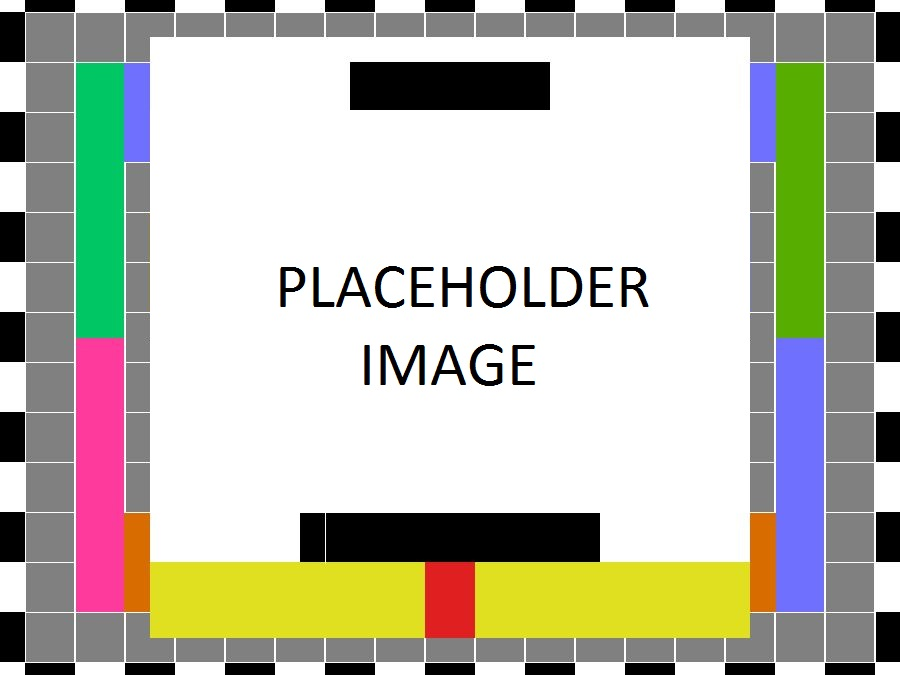
\includegraphics[width=0.60\textwidth]{images/test_image}
\end{figure}
\vspace{0.5 in}
{\centering \huge \color{accentcolor} \sc \textbf{\teamname \\ \productname} \par}
\vspace{0.5 in}
{\centering \large \sc \textbf{\authors} \par}
\newpage


%\vspace{1 in}
%\centerline{January 13th, 2012}
%\newpage

%%% Revision History
\begin{versionhistory}
  	\vhEntry{0.1}{09.26.2019}{HQ|AA|DN|DN|AR}{document creation}
  	\vhEntry{0.2}{09.30.2019}{AA|HQ|DN|DN|AR}{complete draft}
  	\vhEntry{1.0}{10.01.2018}{AA|HQ|DN|DN|AR}{official release}
\end{versionhistory}
\newpage

%%% Table of contents
\setcounter{tocdepth}{2}
\tableofcontents
\newpage

%%% List of figures and tables (optional)
\listoffigures
\listoftables
\newpage

%%% Document sections
\section{Introduction}
Your introduction should provide a brief overview of the product concept and a reference to the requirement specification and architectural design documents in 1 or 2 paragraphs. The purpose is to provide the reader with the location of relevant background material that lead to the design details presented in this document.

\newpage
\section{System Overview}
The application layer will take user inputs and send that input to the hub or the shutters directly depending on the connection type. The application layer is also able to request data from the shutters as well such as the current position and battery level 

\begin{figure}[h!]
	\centering
 	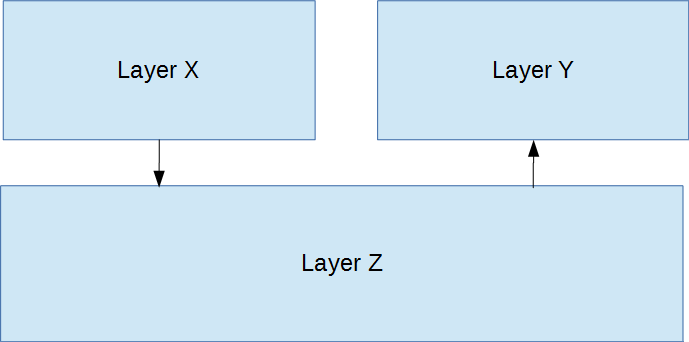
\includegraphics[width=0.60\textwidth]{images/layers}
 \caption{A simple architectural layer diagram}
\end{figure}

\subsection{Layer X Description}
Each layer should be described separately in detail. Descriptions should include the features, functions, critical interfaces and interactions of the layer. The description should clearly define the services that the layer provides. Also include any conventions that your team will use in describing the structure: naming conventions for layers, subsystems, modules, and data flows; interface specifications; how layers and subsystems are defined; etc. 

\subsection{Layer Y Description}
Each layer should be described separately in detail. Descriptions should include the features, functions, critical interfaces and interactions of the layer. The description should clearly define the services that the layer provides. Also include any conventions that your team will use in describing the structure: naming conventions for layers, subsystems, modules, and data flows; interface specifications; how layers and subsystems are defined; etc. 

\subsection{Layer Z Description}
Each layer should be described separately in detail. Descriptions should include the features, functions, critical interfaces and interactions of the layer. The description should clearly define the services that the layer provides. Also include any conventions that your team will use in describing the structure: naming conventions for layers, subsystems, modules, and data flows; interface specifications; how layers and subsystems are defined; etc. 
\newpage
\section{Subsystem Definitions \& Data Flow}
\begin{figure}[h]
	\centering
 	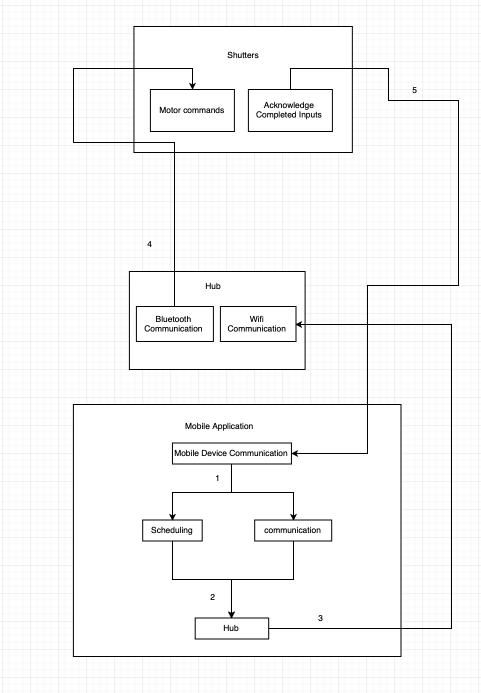
\includegraphics[width=100mm]{images/SysOverview}
 \caption{A simple data flow diagram}
\end{figure}

\newpage
\section{X Layer Subsystems}
\subsection{Layer Hardware}
A mobile phone

\subsection{Layer Operating System}
User’s will need to have Android 10.0 and iOS 13


\subsection{Layer Software Dependencies}
React Native framework

\subsection{Scheduling}
When users want to set a schedule this sub-system will handle the task. The system will send a HTTP post request to the hub which set the schedule, handle the task, and notify users when the task is completed

\begin{figure}[h!]
	\centering
 	\includegraphics[width=0.60\textwidth]{images/mobile}
 \caption{Mobile subsystem layer}
\end{figure}

\subsubsection{Subsystem Hardware}
Users should have either devices Android or iOS.

\subsubsection{Subsystem Operating System}
Android 10.0 or iOS 13 or later

\subsubsection{Subsystem Software Dependencies}
Users be connected to the shutter with Bluetooth or the hub via Wi-Fi and users have not tampered with the Application 

\subsubsection{Subsystem Programming Languages}
Node JS


\subsubsection{Subsystem Data Structures}
Data received by the hub will be in JSON format and request will be HTTP request. Name of the shutter along with the mac address will be stored in a dictionary with the name being the value and the mac address being the key.


\subsubsection{Subsystem Data Processing}
JSON formatting for from the http get request

\subsection{Communication layer}

\subsubsection{Subsystem Hardware}
Users have devices that are running Android 10.0 or iOS 13 or later

\subsubsection{Subsystem Operating System}
Android 10.0 or iOS 13 or later

\subsubsection{Subsystem Software Dependencies}
React native framework
The application must be able to send HTTP get or post request to the hub, also be able to communicate to the shutter through Bluetooth 

\subsubsection{Subsystem Programming Languages}
Node JS

\subsubsection{Subsystem Data Structures}
The application must send an HTTP request to the hub if users are connecting through WiFi 
If users are connected directly to the shutter they must send request through Bluetooth and receive acknowledgement packets

\subsubsection{Subsystem Data Processing}
Using simple HTTP request and bluetooth libraries to communicate 



\newpage
\section{Y Layer Subsystems}
\subsection{Layer Hardware}

Software running on a Raspberry pi 0w with Raspbian Buster / 2020-02-05
The raspberry pi 0w is small, made in large scale, and is only \$10

\subsection{Layer Operating System}
Raspbian Buster / 2020-02-05 current version of raspbian available

\subsection{Layer Software Dependencies}
Django 3.0 web framework
Cronjobs  

\subsection{Bluetooth communication}
Communicate request to the shutters over bluetooth using python the bluetool library

\begin{figure}[h!]
	\centering
 	\includegraphics[width=0.60\textwidth]{images/hub}
 \caption{Hub subsystem}
\end{figure}

\subsubsection{Subsystem Hardware}
Raspberry pi 0W and ESP32

\subsubsection{Subsystem Operating System}
Raspbian Buster / 2020-02-05 the current version of raspbian available

\subsubsection{Subsystem Software Dependencies}
Python Bluetool library

\subsubsection{Subsystem Programming Languages}
Using Python 2.7 to communicate to the shutter

\subsubsection{Subsystem Data Structures}
The hub will receive HTTP user requests and send the commands to the shutters via Bluetooth, then receive acknowledgments from the shutter and send the acknowledgment to the user. 

\subsubsection{Subsystem Data Processing}
Send commands to shutter through Bluetooth using the bluetool python library

\subsection{Wi-Fi communication}
Receiving HTTP request and sending JSON back to the application

\subsubsection{Subsystem Hardware}
Using a Raspberry Pi 0W

\subsubsection{Subsystem Operating System}
Raspbian Buster / 2020-02-05 the current version of raspbian available

\subsubsection{Subsystem Software Dependencies}
Django 3.0 Web framework
Bluetool


\subsubsection{Subsystem Programming Languages}
System will be built on the current version of Python 3 and Python 2.7

\subsubsection{Subsystem Data Structures}
Using a dictionary to contain the mac address as the key and the name as the value of the shutter
Sending data and receiving request from mobile users through HTTP request

\subsubsection{Subsystem Data Processing}
Sending information to mobile applications in JSON format as a HTTP response to application api calls.


\newpage
\section{Z Layer Subsystems}

\subsection{Layer Hardware}
ESP 32

\subsection{Layer Operating System}
Mongoose OS

\subsection{Layer Software Dependencies}
Django 3.0 Web framework
Bluetool


\subsection{Motor commands}
Receive Bluetooth commands and turn the corresponding shutters

\begin{figure}[h!]
	\centering
 	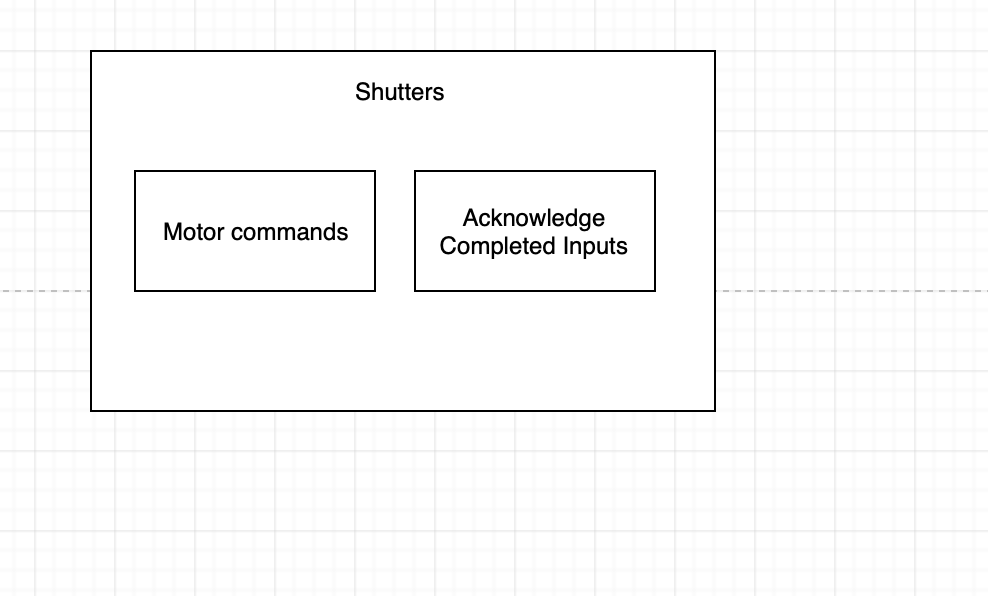
\includegraphics[width=0.60\textwidth]{images/Shutters}
 \caption{Example subsystem description diagram}
\end{figure}

\subsubsection{Subsystem Hardware}
ESP32

\subsubsection{Subsystem Operating System}
Mongoose OS

\subsubsection{Subsystem Software Dependencies}
Django 3.0 Web framework
Bluetool

\subsubsection{Subsystem Programming Languages}
C and micro python

\subsubsection{Subsystem Data Structures}
When the esp32 is given a request it will complete the request and send a message back to the original sender

\subsubsection{Subsystem Data Processing}
Esp32 will receive request and complete the request and send an acknowledgment 

\subsection{Acknowledge Completed Request}
Acknowledge completed Bluetooth commands

\subsubsection{Subsystem Hardware}
ESP32

\subsubsection{Subsystem Operating System}
Mongoose OS

\subsubsection{Subsystem Software Dependencies}
Bluetooth module working and request be formatted properly


\subsubsection{Subsystem Programming Languages}
C and micro python

\subsubsection{Subsystem Data Structures}
After the packets are received the shutter will try to complete the task and send a message back to original sender 

\subsubsection{Subsystem Data Processing}
Input checking making sure the input is properly formatted and checks to see if the new position does not equal the current position






\newpage

%%% References
\bibliographystyle{plain}
\bibliographystyle{reference/IEEEtran_custom}
\bibliography{reference/refs}{}

\end{document}